%%%%%%%%%%%%%%%%%%%%%%%%%%%%%%%%%%%%%%%%%%%%%%%%%%%%%%%%%%%%%%%%%%%%%%%%%%%%%%%%
% Introduction
%%%%%%%%%%%%%%%%%%%%%%%%%%%%%%%%%%%%%%%%%%%%%%%%%%%%%%%%%%%%%%%%%%%%%%%%%%%%%%%%
\subsection{Introduction}
\begin{frame}[label=algorithm-introduction]{Introduction}
        {Anomaly Detection Using Commute Time}
    {\Large \textbf{Anomaly Detection Using Commute Time}}\\

    \medskip
    {\small \fullcite{Khoa:2012}}
    \note{The algorithm that was selected for implementation was developed by
        \citeauthor{Khoa:2012} and published in \citetitle{Khoa:2012}.}

    \bigskip
    \begin{columns}[c]
        \column{0.5\textwidth}
        \begin{figure}[H]
            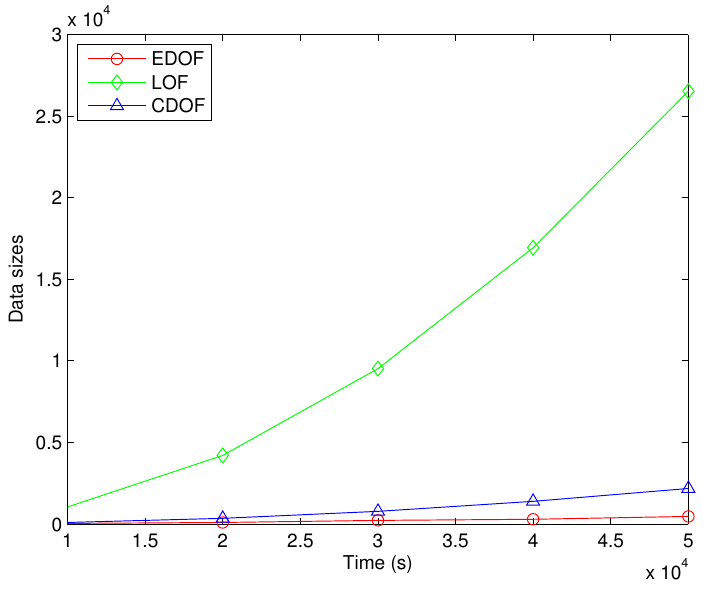
\includegraphics[width=0.7\textwidth]{algorithm/run-time}
            \caption{\scriptsize Execution time of approximate commute time method versus
                Euclidean distance and \gls{LOF} methods}
        \end{figure}

        \column{0.5\textwidth}
        \begin{figure}[H]
            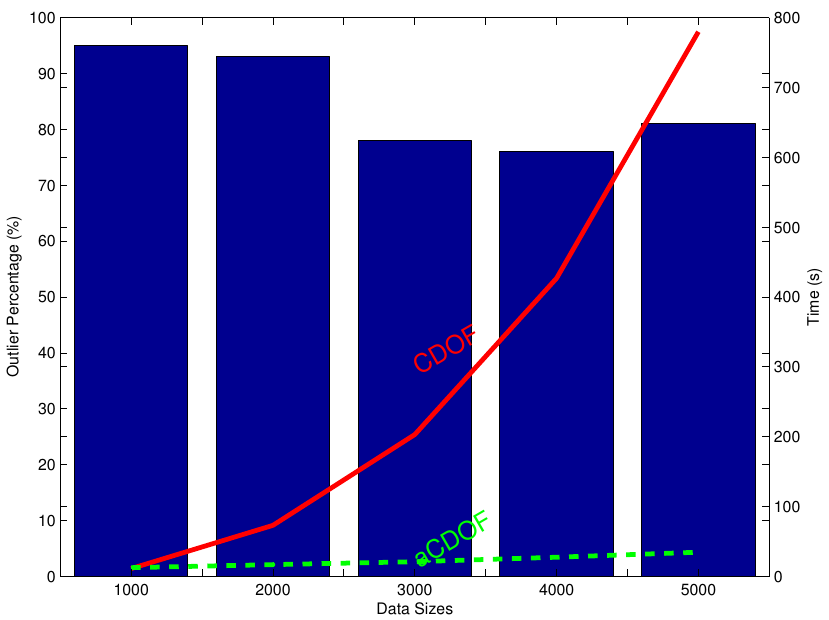
\includegraphics[width=0.7\textwidth]{algorithm/accuracy}
            \caption{\scriptsize Accuracy and execution time of approximated commute
                distance method compared to non-approximated method}
        \end{figure}
    \end{columns}

    \note{
        These graphs show the measured performance of the chosen algorithm.

        \begin{itemize}
            \item The left graph shows how run time (using \emph{approximated}
                commute time) is proportional to $O(n \log n)$, compared to:
            \begin{itemize}
                \item $O(n)$ using Euclidean distance
                \item $O(n^2)$ using \gls{LOF}
            \end{itemize}

            \item The right graph shows how anomaly detection using
                \emph{approximated} commute time preserves a high percentage
                (84.6\% on average) of the top anomalies discovered without
                using approximations.
            \end{itemize}}
\end{frame}

%%%%%%%%%%%%%%%%%%%%%%%%%%%%%%%%%%%%%%%%%%%%%%%%%%%%%%%%%%%%%%%%%%%%%%%%%%%%%%%%
% The Algorithm
%%%%%%%%%%%%%%%%%%%%%%%%%%%%%%%%%%%%%%%%%%%%%%%%%%%%%%%%%%%%%%%%%%%%%%%%%%%%%%%%
\subsection{The Algorithm}
\begin{frame}[label=algorithm]{The Algorithm}
        {Anomaly Detection Using Commute Time}\relax
    {\tiny
        \begin{algorithm}[H]
            % TODO
\LinesNumbered

\SetKwInput{InputK}{k}
\SetKwInput{InputN}{N}
\SetKwInput{InputD}{Data}
\SetKwInOut{OutputO}{outliers}

\InputK{the number of nearest neighbors}
\InputN{the number of outliers to return}
\InputD{a set of examples in random order}
\OutputO{a set of outliers}

\SetKwData{varB}{b}
\SetKwData{Block}{block}
\SetKwData{Cutoff}{cutoff}
\SetKwData{varD}{d}
\SetKwData{Data}{Data}
\SetKwData{varK}{k}
\SetKwData{varN}{N}
\SetKwData{Neighbours}{neighbours}
\SetKwData{varO}{o}
\SetKwData{Outliers}{outliers}
\SetKwData{Score}{score}

\SetKwFunction{Closest}{closest}
\SetKwFunction{Distance}{distance}
\SetKwFunction{GetNextBlock}{getNextBlock}
\SetKwFunction{MaxDist}{maxDist}
\SetKwFunction{Min}{min}
\SetKwFunction{Top}{top}

\Begin{
    $\Cutoff \longleftarrow 0$\tcp*[l]{set the cutoff for pruning to $0$}
    $\Outliers \longleftarrow \emptyset$\tcp*[l]{initialize to the empty set}
    \BlankLine
    \While(\tcp*[h]{load a block of examples from \varD}){$\Block \longleftarrow \GetNextBlock{\Data}$}{
        $\Neighbours(\varB) \longleftarrow \emptyset, \quad \forall \, \varB \in \Block$\;
        \BlankLine
        \ForEach{$\varD \in \Data$}{
            \ForEach{$\varB \in \Block \: : \: \varB \neq \varD$}{
                \If{$|\Neighbours(\varB)| < \varK \: \lor \: \Distance{\varB, \varD} < \MaxDist{\varB, \Neighbours(\varB)}$}{
                    $\Neighbours(\varB) \longleftarrow \Closest{\varB, \Neighbours(\varB)} \cup \varD, \varK)$\;
                    \If{$\Score(\Neighbours(\varB), \varB) < \Cutoff$}{
                        $\Block \longleftarrow \Block \setminus \varB$\;
                    }
                }
            }
        }
        \BlankLine
        $\Outliers \longleftarrow $\Top{$\Block \cup \Outliers$, $\varN$}\tcp*[l]{keep only the top n outliers}
        $\Cutoff \longleftarrow \Min_{\varO \in \Outliers}(\Score(\varO))$\tcp*[l]{the cutoff is the score of the weakest outlier}
    }
    \KwRet{\Outliers}\;
}

        \end{algorithm}}

    \note{The $k$-nearest neighbour graph with $n$ nodes is built in
        $O(n \log n)$ using kd-tree with the assumption that the dimensionality
        of the data is not very high. The average degree of each node is $O(k)$
        ($k << n$). So the graph is sparse and thus finding connected components
        takes $O(kn)$.

        After sampling, the size of graph is $O(n_s)$ ($n_s << n$). The standard
        method for eigen decomposition of $L_s$ is $O(n_s^3)$. Since $L_s$ is
        sparse, it would take $O(Nn_s) = O(kn_s^2)$, where $N$ is the number of
        nonzeros. The computation of just the $m$ smallest eigenvectors
        ($m < n_s$) is less expensive than that.

        The typical distance-based anomaly detection takes $O(n_s^2)$ for the
        neighbourhood search. Pruning can scale it nearly linear. We only need
        to compute the commute times $O(n_s)$ times, each of which takes $O(m)$.
        So the time needed for two steps is proportional to
        $O(n \log n + kn + kn_s^2 + mn_s) = O(n \log n)$ as $n_s << n$.}
\end{frame}

\begin{frame}[label=algorithm]{The Algorithm}
        {Outlier Pruning}\relax
    {\tiny
        \begin{algorithm}[H]
            \LinesNumbered

\SetKwInput{InputK}{k}\InputK{the number of nearest neighbours to consider}
\SetKwInput{InputN}{N}\InputN{the number of outliers to return}
\SetKwInput{InputData}{data}\InputData{a set of examples in random order}
\SetKwInOut{Output}{outliers}\Output{a set of outliers}
\SetKwInOut{OutputScores}{outlier\_scores}\OutputScores{}

\SetKwData{BlockIterator}{b}
\SetKwData{Block}{block}
\SetKwData{Cutoff}{cutoff}
\SetKwData{DataIterator}{d}
\SetKwData{Data}{data}
\SetKwData{NumK}{k}
\SetKwData{NumN}{N}
\SetKwData{Neighbours}{neighbours}
\SetKwData{OutlierIterator}{o}
\SetKwData{Outliers}{outliers}
\SetKwData{Score}{score}

\SetKwFunction{Closest}{closest}
\SetKwFunction{Distance}{distance}
\SetKwFunction{LoadBlock}{load\_next\_block}
\SetKwFunction{MaxDist}{max\_dist}
\SetKwFunction{Min}{min}
\SetKwFunction{Top}{top}

\Begin{
    \Cutoff $\leftarrow$ 0\tcp*[l]{set the cutoff for pruning to $0$}
    \Outliers $\leftarrow\emptyset$\tcp*[l]{initialize to the empty set}
    \BlankLine
    \While(\tcp*[h]{load a block of examples from \Data}){\Block $\leftarrow$ \LoadBlock{\Data}}{
        \ForEach{\BlockIterator $\in$ \Block}{
            $\Neighbours[\BlockIterator]\leftarrow\emptyset$\;
        }
        \BlankLine
        \ForEach{\DataIterator $\in$ \Data}{
            \ForEach{\BlockIterator $\in$ \Block $:$ \BlockIterator $\neq$ \DataIterator}{
                \If{$|\Neighbours[\BlockIterator]|<$ \NumK $\:\lor\:$ \Distance{\BlockIterator, \DataIterator} $<$ \MaxDist{\BlockIterator, $\Neighbours[\BlockIterator]$}}{
                    %$\Neighbours[\BlockIterator] \leftarrow$ \Closest{\BlockIterator, $\Neighbours[\BlockIterator]$} $\cup$ \DataIterator,\NumK)$\;
                    \If{$\Score[\Neighbours[\BlockIterator],\BlockIterator)<\Cutoff$}{
                        \Block $\leftarrow$ \Block $\setminus$ \BlockIterator\;
                    }
                }
            }
        }
        \BlankLine
        \Outliers $\leftarrow$ \Top{\Block $\cup$ \Outliers, \NumN}\;
        \Cutoff $\leftarrow$ $\Min_{\OutlierIterator \in \Outliers}(\Score(\OutlierIterator))$\tcp*[l]{the cutoff is the score of the weakest outlier}
    }

    \BlankLine
    \KwRet{\Outliers}\;
}

        \end{algorithm}}
\end{frame}

\begin{frame}[label=algorithm-animation]{Animation}
        {A short animation illustrating the algorithm execution}
    \centering
    \movie[once,showcontrols]
        {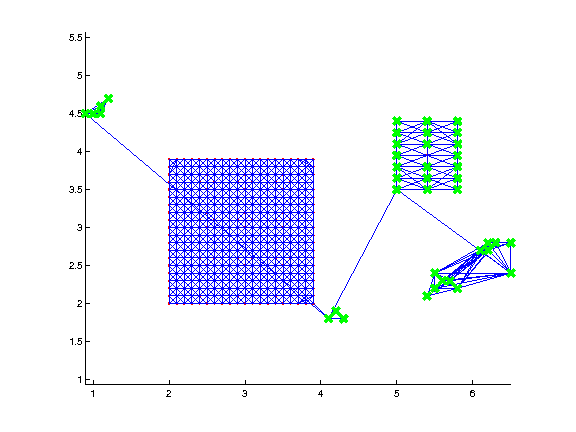
\includegraphics[width=0.8\textwidth]{pca/testoutrank}}
        {animation/testoutrank.avi}

    \note{This slide shows a short animation, illustrating the execution of the
        chosen anomaly detection method on a data set of 441 2-dimensional
        vectors.

        In this animation, the yellow points indicate the current block that is
        being processed. Each vector within the block is compared to all other
        vectors in the data set, illustrated by the blue marker in the
        animation.

        Each vector in the current block is given a score, a monotonic
        decreasing function that provides a heuristic to estimate if any given
        vector may be an outlier.

        The current `best' outliers are highlighted in green in the animation.
        As the algorithm processes further blocks of data, the set of current
        outliers converges to the final set of outliers.

        If the score for any vector in the current block becomes less than the
        lowest score from the set of current outliers, then this vector is no
        longer considered to be a possible outlier, and is pruned from the data
        set. The pruned vectors appear in red in the animation.}
\end{frame}
